\documentclass[12pt]{report}

%Packages-------------------------------------
\usepackage{amsmath}
\usepackage{amsfonts}
\usepackage{amssymb}
\usepackage{amsthm}
\usepackage{graphics}
\usepackage{graphicx}
\usepackage{float}
\usepackage{adjustbox}
 \usepackage[stable]{footmisc}
\usepackage{setspace}
\usepackage{adjustbox}
%\usepackage{hyperref}
\usepackage{pgfplots}
%\usepackage{xtocnic}
\usepackage{nameref}
\usepackage{listings}
\usepackage{caption}
\usepackage{xepersian}

\lstset{
basicstyle=\small\ttfamily,
columns=flexible,
breaklines=true
}
\settextfont{XB ZAR.TTF}
\renewcommand\bibname{مراجع}


%Layout---------------------------------------

%\usepackage[top=2cm, bottom=2cm, left=2cm, right=2cm]{geometry}

%Commands-------------------------------------


%Theorems-------------------------------------

\begin{document}

%Title page ---------------------------------------------

\begin{figure}
\centering
\includegraphics[height=2.5cm]{UT-Logo.pdf}
\end{figure}

\begin{center}
پردیس علوم
\\
دانشکده‌ی ریاضی، آمار و علوم کامپیوتر
\end{center}

\begin{center}
%%%%%%%%%%%%%
\end{center}

\begin{center}
\huge{ تحلیل داده‌های بازار بورس ایران با استفاده از الگوریتم‌های داده‌کاوی}
\end{center}

\begin{center}
%%%
\end{center}

\begin{center}
نگارنده
\end{center}
\begin{center}
\textbf{
محمدحسین خوش رفتار
}
\end{center}

\begin{center}
\begin{tabular}{rr}
استاد راهنما: دکتر سمانه افتخاری مهابادی
\end{tabular}
\end{center}

\vspace{3cm}
\begin{center}
پایان‌نامه برای دریافت درجه کارشناسی
\\
در رشته علوم کامپیوتر
\end{center}

\begin{center}
تیر ۱۴۰۰
\end{center}

\pagestyle{empty}
\pagenumbering{}

\newpage
%\pagestyle{headings}
%\setcounter{page}{1}
%\pagenumbering{roman}
\pagestyle{plain}
\setcounter{page}{1}
\pagenumbering{harfi}
%Abstract page-------------------------------
\doublespacing{}
\chapter*{}
\section*{چکیده}
هدف این پروژه پیش بینی وضعیت سهم‌های بازار بورس تهران با استفاده از تاریخچه ی سهم و سایر شاخص های اقتصادی از جمله قیمت دلار ، تورم ، نقدینگی و … می‌باشد. با استفاده از روش ها و الگوریتم های داده کاوی سعی کردیم که به کمک تاریخچه ی سهم و شاخص های اقتصادی مهم به مدلی دست پیدا کنیم که آینده ی سهم را پیش بینی کند. در گام نخست داده‌های مورد نیاز راجمع آوری کردیم. داده‌های سال ۲۰۱۵ تا سال ۲۰۲۰ از تمامی سهم ها و شاخص های اقتصادی نام برده شده را با فرمت csv ذخیره کردیم. در گام بعدی با رسم نمودار های مناسب و تحلیل شاخص ها کنار هم به بررسی اینکه کدام شاخص ها بر قیمت سهم تاثیر گذارند پرداختیم و شاخص های مناسب را انتخاب کردیم. در گام آخر هم با استفاده از داده‌های موجود به بررسی و تست مدل های مناسب جهت پیش بینی سری های زمانی با دقت مناسب پرداختیم و در نهایت با استفاده از
مدل میانگین متحرک خود همبسته یکپارچه
\LTRfootnote{\lr{ARIMA model}}
یک مدل جهت پیش بینی قیمت سهم ها آموزش دادیم و دقت سنجی کردیم.

\chapter*{پیشگفتار }


مهم ترین مسئله در بازار سرمایه پیش‌بینی آینده سهم است. با مشخص شدن وضعیت سهم در آینده ، استراتژی خرید و فروش به آسانی به دست می آید و می توانیم میزان سود را ماکزیمم کنیم. فاکتور های بسیار زیادی بر قیمت سهم تاثیر گذار هستند. مهم ترین فاکتور ها عملکرد مالی شرکت صاحب سهم و تاریخچه ی خود سهم هستند ولی از آنجایی که در کشور وضعیت شاخص های اقتصادی پایدار نیست ، عواملی چون قیمت دلار ، تورم ، نقدینگی و … تاثیر زیادی روی قیمت سهم ها می گذراند. ازین‌رو برای پیش بینی قیمت سهم نیازمند مدلی هستیم که علاوه بر توجه به تاریخچه‌ی سهم یا همان ویژگی های سری های زمانی به تاریخچه ی دیگر شاخص های اقتصادی نیز توجه نماید و تغییرات آن ها را در تصمیم گیری لحاظ کند. یکی از چالش های مهم این راه یکسان نبودن واحد و مقیاس در شاخص های اقتصادی مذکور می‌باشد که باعث ایجاد خطا در مدل و تصمیم گیری خواهد شد که باید با استفاده از نرمال سازی و تبدیل های مناسب این مشکل را برطرف کرد.
در زمینه‌ی پیش‌بینی قیمت سهم مقالات زیادی وجود دارد ولی اکثرا به شاخص های اقتصادی و تاثیرات آن‌ها نپرداخته‌اند و تمرکز را روی تحلیل سری زمانی خود سهم و الگوی افزایش و کاهش قیمت قرار داده‌اند. به طور مثال در سال ۲۰۱۵ اقای اگاندی در مقاله‌ای [3]
به کمک مدل‌های داده کاوی از جمله مدل ARIMA به تحلیل داده‌های بورسی پرداخته است.
در این پروژه سعی شده است که تاثیرات شاخص های اقتصادی اعمال شود.

\tableofcontents


\chapter{مقدمه}

\pagestyle{plain}
\setcounter{page}{1}
\pagenumbering{arabic}
پروژه از ۳ فاز اصلی تشکیل شده که به ترتیب جمع آوری و پیش پردازش داده، بررسی شهودی و انتخاب پیشگو ها و در نهایت طراحی و پیاده سازی مدل می باشد.
تمام مراحل فنی این پروژه با استفاده از
زبان برنامه نویسی پایتون
\LTRfootnote{Python programming language}
 پیاده سازی شده است و تمام مراحل پیاده سازی پروژه تحت
 گیت
\LTRfootnote{\lr{Git}}
ثبت شده است و میتوانیم مراحل و تاریخچه را به کمک آن ببینیم.
به منظور تصمیم بهتر راجع به
پیشگو
\LTRfootnote{\lr{Predictor}}
های اقتصادی مطرح شده نیاز است که به طور شهودی با آن ها آشنا باشیم که در ادامه به طور مختصر توضیحاتی راجع به آن ها فراهم شده است.
علاوه بر این برای فهم بهتر تحلیل های ارائه شده خوب است که با مفاهیم اولیه ی بازار بورس آشنا باشیم ولی به دلیل گستردگی این مطالب از اشاره به همه ی آن ها خودداری کرده ایم و فقط به موارد ضروری اشاره شده است.

\section{مفاهیم}
\subsection{قیمت دلار}
در این پروژه منظور از قیمت دلار ، ارزش یک دلار آمریکا به ریال در تاریخ مشخصی و با توجه به قیمت رسمی اعلام شده از سوی بانک مرکزی می باشد.
\subsection{تورم}
تورم
\LTRfootnote{Inflation}
 نرخ تغییر سطح عمومی قیمت‌ها می باشد و بر اساس میانگین تغییرات قیمت مجموعه ای از کالاهای مشخصی محاسبه می‌شود. شاخص تورم به صورت ماهانه توسط بانک مرکزی و همچنین سازمان آمار محاسبه و اعلام می شود.
در این پروژه از آمار رسمی که توسط سازمان آمار اعلام می شود استفاده شده است.
\subsection{نقدینگی}
نقدينگي
\LTRfootnote{Cash}
مجموع پول و شبه پولي است كه در اقتصاد كشور جريان دارد. پول، طبق تعريف شامل اسكناس و مسكوك در دست اشخاص به علاوه سپرده‌هاي ديداري است و شبه پول نيز شامل سپرده‌هاي غيرديداري است. نقدينگي در اقتصاد ضريبي از پايه پولي است كه توسط بانك مركزي خلق شده است.
\par
عوامل موثر بر حجم نقدينگي در اقتصاد عمدتا شامل سه قلم «خالص دارايي‌هاي خارجي سيستم بانكي»، «خالص بدهي بخش دولتي به سيستم بانكي» و «بدهي بخش غيردولتي به سيستم بانكي» است. مجموع اقلام فوق به صورت پول و شبه‌پول در اقتصاد به گردش درمي‌آيد.
\subsection{تاریخچه قیمت}
منظور از تاریخچه ی قیمت،
سری زمانی
\LTRfootnote{\lr{Time series}}
قیمت سهم می باشد. یعنی اینکه به ازای هر روز خاص قیمت سهم در اون روز چقدر بوده است.
معمولا در بازار بورس تهران قیمت پایانی سهم به عنوان قیمت سهم در یک روز خاص در نظر گرفته می‌شود ولی به طور کلی در بقیه بازار ها معمولا از آخرین قیمت استفاده می‌شود.
\subsection{قیمت پایانی}
منظور از
قیمت پایانی
\LTRfootnote{\lr{Closing price}}
 یک روز، میانگین وزن دار تمام معاملات آن روز با وزن حجم معاملات انجام شده می باشد.
 در بازار بورس تهران با توجه به اینکه محدودیت قیمت برای سهم‌ها وجود دارد قیمت پایانی اهمیت پیدا می‌کند زیرا تعیین کننده‌ی محدوده نوسانی قیمت روز معاملاتی آینده می‌باشد.
 \par
 محدوده نوسانی قیمت هر سهم در هر روز معاملاتی معمولا بازه‌ی ۵ درصد کمتر تا ۵ درصد بیشتر از قیمت پایانی روز معاملاتی گذشته است.

\subsection{آخرین قیمت}
منظور از آخرین قیمت هر سهم، قیمت آخرین معامله‌ی انجام شده‌ی سهم در روز معاملاتی مشخصی می‌باشد.
این قیمت مستقل از حجم معامله‌انجام شده می‌باشد.

\subsection{پیشگو}
پیشگو متغیری می‌باشد که جهت پیش‌بینی متغیری دیگر که به عنوان متغیر هدف شناخته می‌شود استفاده می‌شود.متغیر پیشگو معادل متغیر مستقل در علم ریاضیات می‌باشد.
برای پیش‌بینی متغیر هدف ممکن است چندین پیشگو وجود داشته باشد.پیشگو ها می‌توانند کاملا مستقل از یکدیگر یا وابسته به هم باشند.

\subsection{متغیر هدف}
متغیر هدف متغیری است که با استفاده از پیشگوها پیش‌بینی می‌شود.
متغیر هدف معادل متغیر وابسته در علم ریاضیات می‌باشد.
از پیشگوهایی که متغیر هدف به آن ها وابسته است جهت پیش‌بینی استفاده می‌شود و مابقی کنار گذاشته می‌شوند.

\subsection{مدل}
در این پروژه، منظور از مدل، مدل آماری می‌باشد. مدل آماری نوعی از مدل ریاضی می‌باشد که دارای مجموعه ای از فرض‌های آماری می‌باشد و روابط بین متغیر های تصادفی را فرمول بندی می‌کند.
مدل‌های آماری کاربرد های فراوانی دارند که در این پروژه برای پیش‌بینی مورد استفاده قرار می‌گیرند.

\subsection{پیش‌بینی}
در این مطالعه، منظور از پیش‌بینی بدست آوردن مقادیر متغیر‌های هدف به کمک متغیر های پیشگو می‌باشد.

\subsection{خطای پیش‌بینی}
منظور از خطای پیش‌بینی اختلاف مقدار واقعی متغیر هدف با مقدار پیش‌بینی شده می باشد در وضعیت مشخصی می‌باشد. این مقدار میتواند صفر باشد و به معنای این است که خطایی وجود نداشته است.

\subsection{داده‌های گم شده}
منظور از
داده‌های گم شده
\LTRfootnote{Missing data}
داده‌هایی می‌باشد که برا اثر خطای نمونه گیری یا سیستمی از دست رفته باشند و قابل دست‌یابی نباشند.
به طور مثال برای داده‌های سهم‌های بورسی ممکن است قیمت بعضی روز‌ها به دلایلی موجود نباشد که به آن داده‌ی گم شده می‌گویند و نیازمند اقدامات خاص خود می‌باشد.

\subsection{بازه زمانی}
در این پروژه منظور از
بازه زمانی
\LTRfootnote{Time interval}
، فاصله‌ی نقاط محور x در سری زمانی مورد بحث می‌باشد. به طور مثال در داده های بورس اگر قیمت روزانه‌ی سهم ها را در نظر بگیریم بازه زمانی مورد بررسی روز می‌شود و اگه قیمت ماهانه سهم‌ها را در نظر بگیریم بازه زمانی مورد بررسی ماه می‌شود.
\chapter{مراحل فنی پروژه}

\section{جمع آوری و پیش پردازش داده ها}
برای هر نوع تحلیل داده کاوی ما نیازمند داده هستیم. بدون داده هیچ تحلیلی هم امکان پذیر نیست. همچنین این داده می بایست یک سری ویژگی ها داشته باشد که تحلیل را آسان تر و دقیق تر کند ازینرو قبل از تحلیل داده و یا مدل سازی آن نیازمند اقداماتی هستیم که در ادامه مورد بحث قرار گرفته اند.
\subsection{جمع آوری داده بورس}
برای تحلیل  ما نیازمند تاریخچه ی سهم های بازار بورس ، تاریخچه ی قیمت دلار ، تورم و نقدینگی بودیم. برای دسترسی به داده‌ی تاریخچه ی سهم های بازار بورس راه های فراوانی هست و ما از کتابخانه ای در زبان پایتون به نام
pytse\_client
استفاده کردیم که قابلیت دانلود تاریخچه ی تمام سهم های بازار سرمایه را به دقت روز از سال ۲۰۱۵ را در اختیارمان قرار میدهد. خروجی استفاده از این کتابخانه یک فایل csv به ازای هر سهم بازار می باشد که حاوی تاریخچه ی سهم مورد نظر با دقت روز می باشد.
این فایل ها در پوشه ی tickers\_data از پروژه قرار دارند.
 به این نکته توجه شود که قیمت پایانی سهم به عنوان قیمت آن روز سهم در نظر گرفته شده است.
\subsection{جمع آوری داده‌های شاخص های اقتصادی}
برای جمع آوری داده‌های تاریخچه ی قیمت دلار از
منبع شبکه ی اطلاع رسانی قیمت ارز
\LTRfootnote{\lr{tgju}}
استفاده شد و قیمت دلار به صورت ماهانه در فایل با فرمت csv ذخیره گردید.
برای سایر شاخص های اقتصادی نام برده شده از منبع مرکز آمار و بانک مرکزی استفاده گردید و داده‌ی ماهانه ی شاخص های مذکور در فایل با فرمت csv با اسامی مشخص هر شاخص ذخیره گردید که در ادامه مورد استفاده قرار گیرد.

\subsection{ حذف نوسانات مقطعی داده}
در گام نخست به منظور ساده تر شدن تحلیل و حذف نوسان های مقطعی، سطح دقت یا بازه‌ی زمانی داده را از روزانه به ماهانه تغییر دادیم بدین شکل که به ازای هر سهم و یا شاخص اقتصادی به جای اینکه به ازای هر روز قیمت را نگه داریم به ازای هر ماه قیمت ابتدا یا انتهای آن ماه را ذخیره کنیم.


\subsection{رسیدگی به داده های گم شده}

با توجه به اینکه نماد های بازار بورس  بر اثر افشا ها یا سایر موارد ممکن است روز هایی بسته باشند و داده در آن روز ها موجود نباشد ، ممکن است در تحلیل ها ما را دچار مشکل کنند و این مسئله باید رسیدگی شود. ازین رو از روش
جاینهی آخرین مشاهده
\LTRfootnote{\lr{last observation carried forward}}
برای پر کردن جای خالی این روز ها استفاده کردیم. بدین شکل که قیمت اولین روزی که سهم بعد از بسته بودن باز شده و تعیین قیمت شده است را به جای روز های بسته بودن سهم قرار می دهیم

\subsection{یکسان سازی مقیاس ها}
با توجه به اینکه مقیاس سهم های بازار سرمایه ، قیمت دلار و سایر شاخص های اقتصادی تفاوت بسیار زیادی دارد و این تفاوت در مقیاس باعث ایجاد خطا در تحلیل ها و کاهش عملکرد مدل می شوند، به جای استفاده از مقدار متغییر ها از درصد تغییر شاخص ها برای تحلیل استفاده کردیم. درصد تغییر در سهم های بازار بورس به همان معنی بازدهی ماهانه سهم هستند و در سایر شاخص ها هم درصد تغییر شاخص در ماه مورد نظر هستند.
\subsection{یکسان سازی مولفه ی x داده}
روشی که ما برای رسیدگی به داده های گم شده انتخاب کردیم باعث میشد که مولفه ی x داده که از جنس تاریخ بود در بعضی از ماه ها یکسان نباشد بدین شکل که در حالت عادی روز اول ماه هست ولی در حالتی که جای گذاری اتفاق افتاده روز دوم سوم یا جلوتر از ماه باشد و این تفاوت در مرحله ی پیاده سازی مدل مشکلاتی به وجود آورد برای همین به جای نگهداری روز در مولفه ی x داده مستقیما ماه مورد نظر رابه عنوان مولفه ی  x در نظر گرفتیم. به طور مثال تاریخ 2019-04-03 به 2019-04 تغییر کرد

\section{تحلیل پیشگو ها}
اکنون که داده‌ها آماده و تمیز شده است نیازمند این هستیم که پیشگو هایی که انتخاب کرده ایم را بررسی نماییم تا از بین پیشگو های مورد نظر فقط آن هایی که روی متغییر هدف ما تاثیر گذار هستند  را به مرحله ی طراحی مدل ببریم. لازم به ذکر است که تاریخچه ی خود سهم با توجه به شناختی که از داده داریم پیشگویی اجتناب ناپذیر می باشد و بدون تحلیل به مرحله مدل سازی میبریم. از ابزار های ترسیمی آمار جهت تحلیل پیشگو ها استفاده کردیم. به منظور رسم نمودار های مورد نیاز از کتابخانه ی پایتونی matplotlib استفاده کردیم.

\subsection{بررسی تاثیر قیمت دلار}
از بین سهم های بازار بورس نماد های فولاد، اخابر و خودرو را به نمایندگی از شاخص های بزرگ جهت تحلیل انتخاب میکنیم.
ابتدا
نمودار سری زمانی
\LTRfootnote{\lr{Time series plot}}
قیمت دلار را در کنار سهم های مذکور مورد بررسی می نماییم.
در شکل
\ref{dollar}
نمودار سری زمانی قیمت دلار به صورت ماهانه ترسیم شده است و در شکل های
\ref{foolad}
و
\ref{akhaber}
نمودار های سری زمانی سهم های فولاد و اخابر ترسیم شده است.
\begin{figure}[H]
\centering
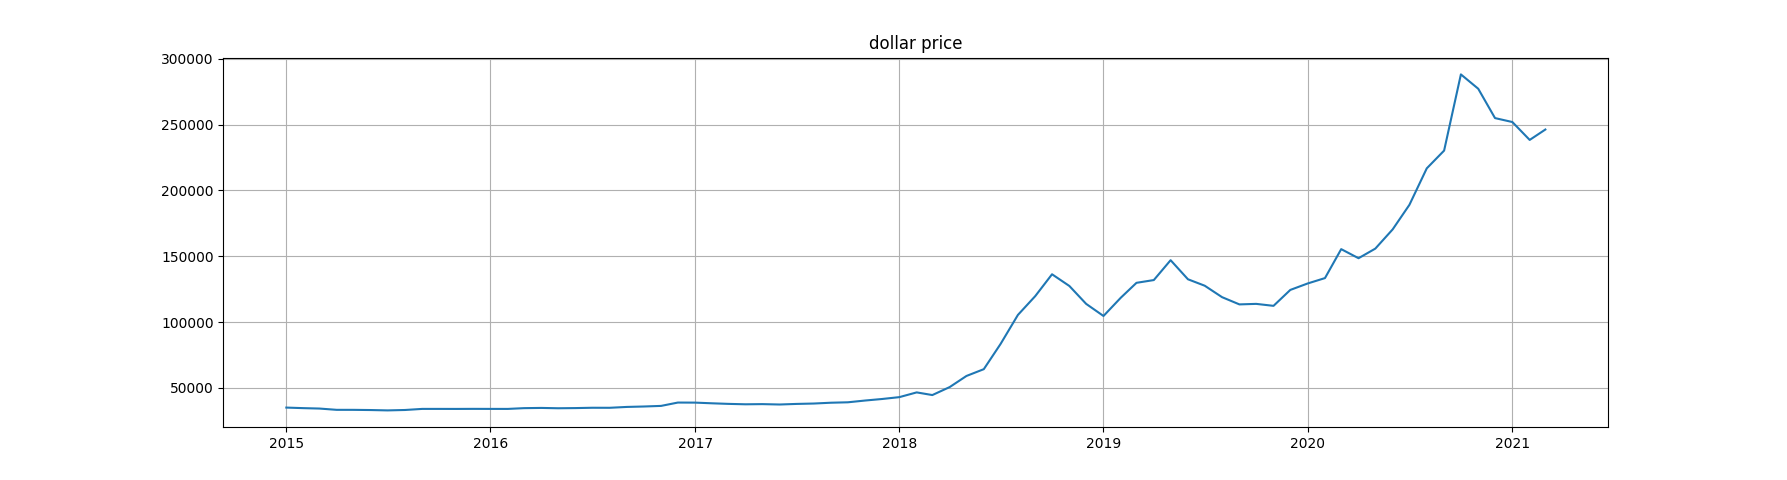
\includegraphics[width=1\textwidth] {new_dollar.png}
\caption{
نمودار قیمت دلار
}
\label{dollar}
\end{figure}
\begin{figure}[H]
\centering
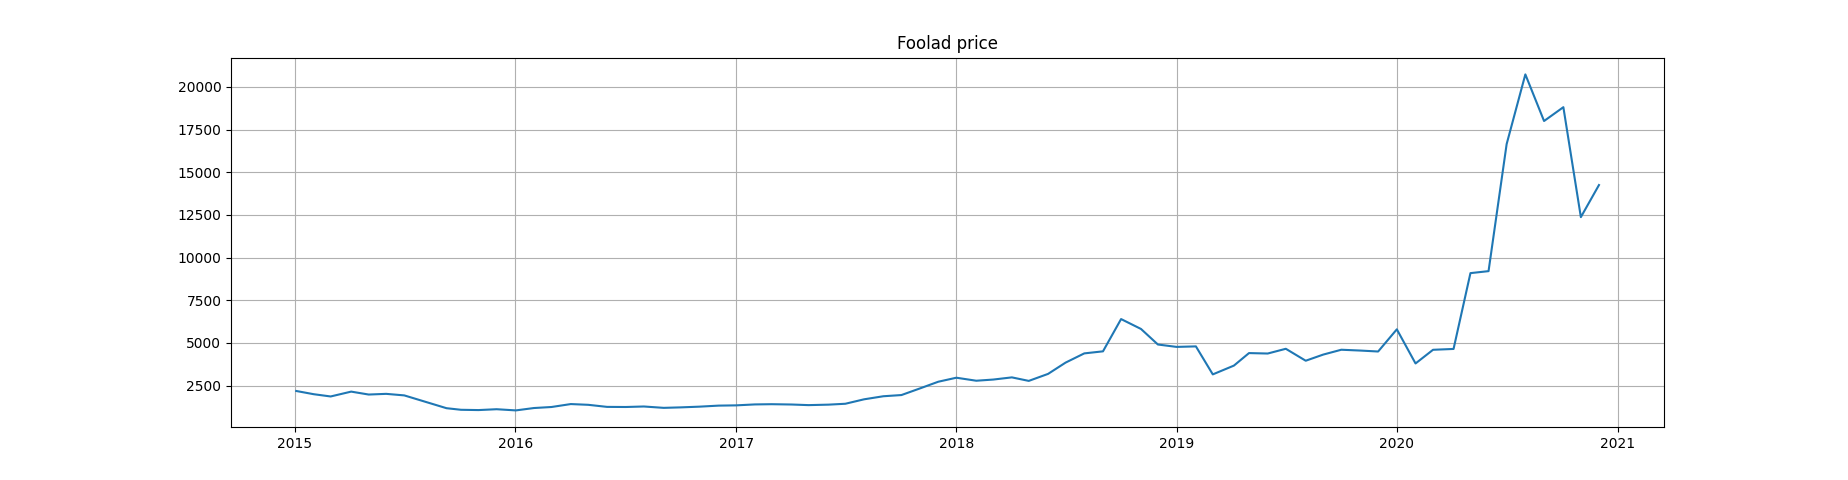
\includegraphics[width=1\textwidth] {new_foolad.png}
\caption{
نمودار قیمت سهم فولاد
}
\label{foolad}$•$
\end{figure}
\begin{figure}[H]
\centering
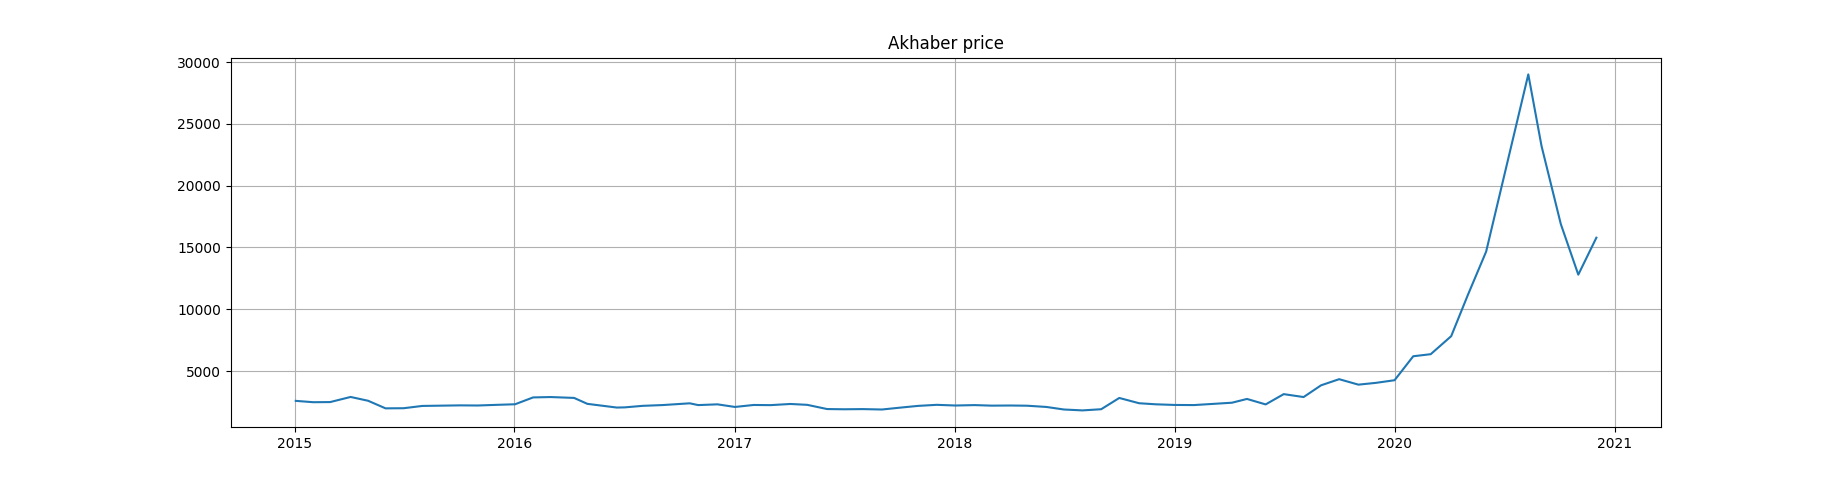
\includegraphics[width=1\textwidth] {new_akhaber.png}
\caption{
نمودار قیمت سهم اخابر
}
\label{akhaber}$•$
\end{figure}
همانطور که مشاهده میشود همبستگی بسیار زیاد بین قیمت دلار و قیمت نماد فولاد و نماد اخابر وجود دارد. با رسم نمودار تغییرات این دو نیز دقیقا به همین نتجیه خواهیم رسید پس از رسم مجدد آن صرف نظر میکنیم.
پس با توجه به تحلیل بالا شواهد کافی برای حضور قیمت دلار در مرحله طراحی مدل وجود دارد.
در ادامه برای تایید شهود ارائه شده شواهد کافی ارائه خواهد شد.
\subsubsection{بررسی تاثیر تورم}
طبق تحلیل شناختی از داده، قابل حدس می باشد که تورم و قیمت دلار به یک معنی هستند و باید یکدیگر را تایید کنند. به منظور اطمینان بیشتر از صحت حدس خود نمودار های تغییرات دلار و تغییرات تورم را در کنار یکدیگر مورد بررسی قرار می دهیم. در شکل
\ref{dollar_change}
نمودار بازدهی دلار که به معنای درصد تغییرات قیمت دلار نسبت به ماه قبل می باشد ترسیم شده است و در ادامه در شکل
\ref{inflation_change}
نمودار بازدهی تورم که به معنای درصد تغییرات تورم ماهانه می باشد ترسیم شده است.
\begin{figure}[H]
\centering
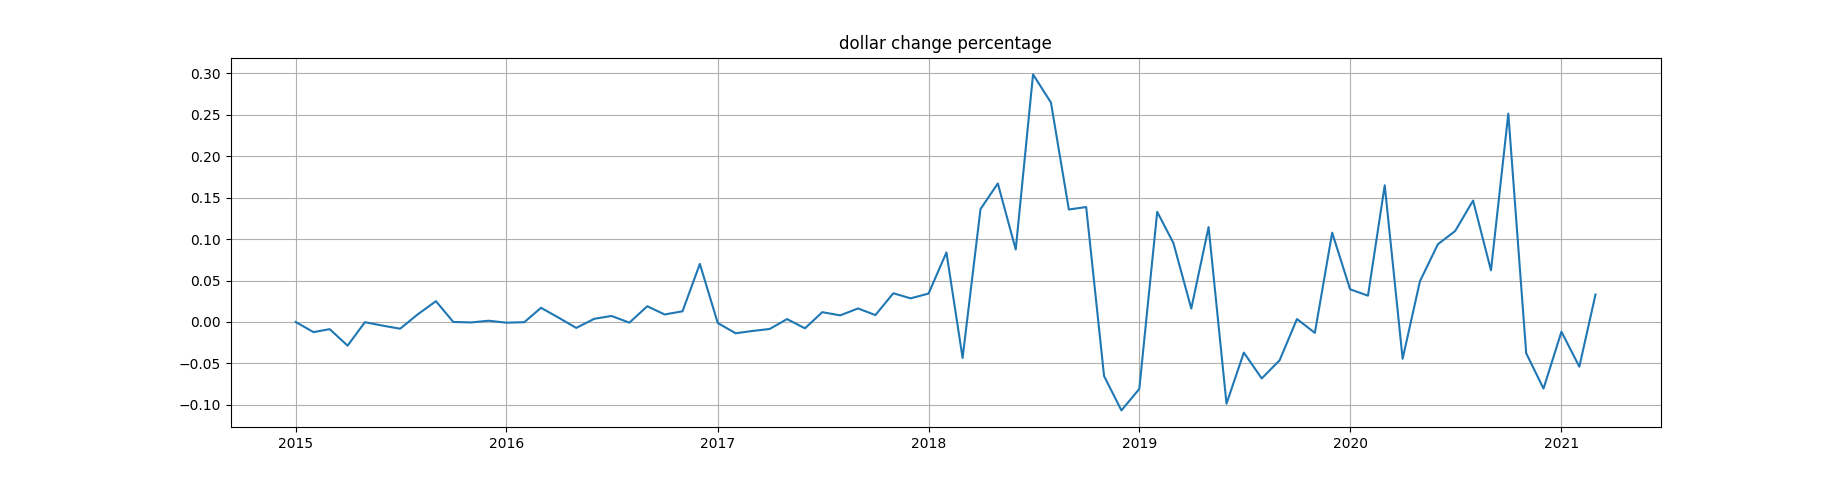
\includegraphics[width=1\textwidth] {new_dollar_change.png}
\caption{
نمودار درصد تغییر قیمت دلار
}
\label{dollar_change}$•$
\end{figure}
\begin{figure}[H]
\centering
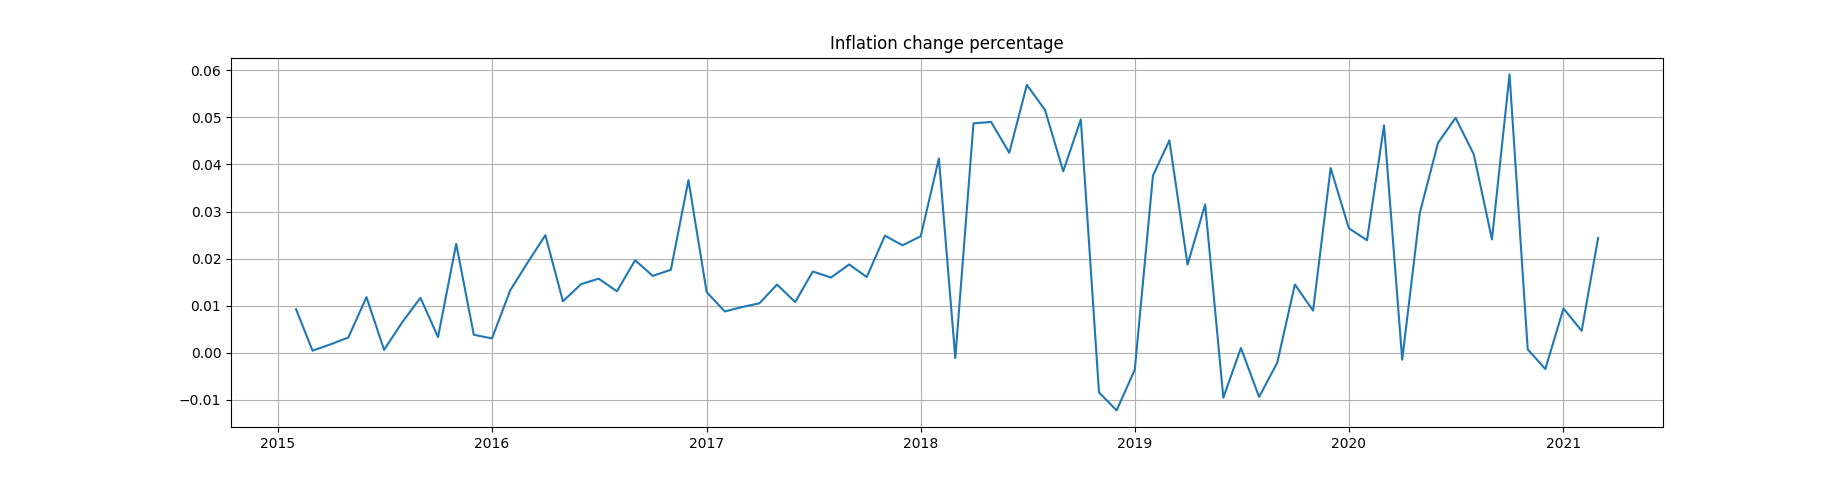
\includegraphics[width=1\textwidth] {new_inflation_change.png}
\caption{
نمودار درصد تغییر تورم
}
\label{inflation_change}$•$
\end{figure}
همانطور که مشاهده می شود تا حد خوبی این دو شاخص با هم همبستگی دارند ولی برای اثبات شهود خود از ضریب همبستگی پیرسون استفاده میکنیم.
جزئیات بیشتر راجع به همبستگی و ضریب همبستگی پریسون در کتاب داده کاوی لارس [1] ذکر شده است.
طبق رابطه زیر  r رامحاسبه میکنیم
\begin{equation*}
r = \frac{\sum{(x_i-\bar{x})*(y_i-\bar{y})}}{\sqrt{\sum{(x_i-\bar{x})^2*\sum(y_i-\bar{y})^2}}}
\end{equation*}
در نهایت با محاسبه r برای داده‌ی  مذکور به عدد ۸۲ صدم با پی مقدار بسیار پایین می‌رسیم که نشان دهنده همبستگی مثبت خوبی هست.
با توجه به همبستگی بالای این دو شاخص میتوان از یکی آن ها در مرحله ی طراحی مدل صرف نظر کرد ولی ممکن است به هر حال یک سری اطلاعات را از دست بدهیم چون همبستگی کامل نداشتن این دو شاخص. با توجه به حجم کم داده، شاخص تورم را نیز در مرحله ی طراحی مدل قرار می دهیم.
\par
برای تایید شهود های ارائه شده در این بخش در جدول
\ref{table}
مقادیر همبستگی شاخص های مختلف گردآوری شده است.


\begin{table}[]
\centering
\begin{latin}
\begin{tabular}{|l|l|l|l|l|l|}
\hline
          & foolad & akhaber & dollar & inflation & cash  \\ \hline
dollar    & 0.787  & 0.775   & 1      & 0.820     & 0.013 \\ \hline
inflation & 0.680  & 0.710   & 0.820  & 1         & 0.025 \\ \hline
cash      & 0.023  & 0.033   & 0.013  & 0.025     & 1     \\ \hline
\end{tabular}
\end{latin}
\caption{همبستگی پیرسون}
\label{table}
\end{table}

از آنجایی که تعداد اعضا ثابت و بزرگ می باشد مقادیر
پی-مقدار
\LTRfootnote{p-value}
ها برای عدد های همبستگی نزدیک ۱ به شدت به صفر نزدیک می باشد و برای عدد های نزدیک به صفر عددی به شدت نزدیک به ۱ می باشد در نتیجه معنا داری اعداد بالا بدیهی می باشد.
\par
در ادامه با بررسی نمودار نقدینگی علت عدد پایین همبستگی هم متوجه می شویم همچنین با توجه به توضیحات قسمت قبل مبنی بر اینکه دلار و تورم باید یکدیگر را تایید نمایند با مشاهده عدد همبستگی نزدیک ۸ دهم، این جمله تایید میشود.

\subsection{بررسی تاثیر نقدینگی}
\begin{figure}[H]
\centering
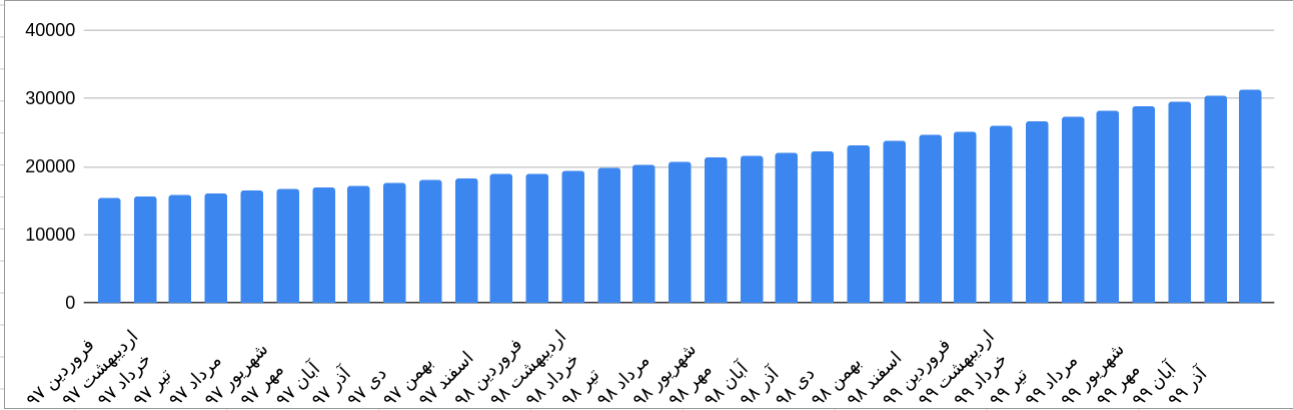
\includegraphics[width=1\textwidth] {cash.png}
\caption{
نمودار نقدینگی ماهانه
}
\label{cash}$•$
\end{figure}
با توجه به نمودار نقدینگی ماهانه متوجه میشویم که نقدینگی کاملا به صورت خطی در حال افزایش است و نوسان خاصی هم ندارد. این به این معنی هست که نقدینگی هیچ اطلاعات ارزشمندی به ما نمی‌دهد. با ترسیم نمودار تغییرات نقدنگی یک خط موازی با محور x ها دریافت میکنیم و همبستگی پایینی هم بین نقدنگی و قیمت سهم ها و دلار وجود خواهد داشت. پس میتوان از ورود شاخص نقدینگی به مرحله ی مدل سازی صرف نظر کرد ولی با توجه به کم بودن حجم داده تصمیم بر این شد که نقدینگی هم وارد مرحله مدل سازی شود که مطمئن شویم اطلاعاتی از دست نمی رود و تحلیل بیشتر این شاخص را به مدل می سپاریم.

\section{انتخاب مدل پایه}
بعد از تحلیل و انتخاب پیشگو ها با توجه به جنس  و
خصیصه
\LTRfootnote{\lr{Feature}}
های داده باید به بررسی مدل های پایه و موجود بپردازیم و با استفاده از یک مدل پایه مدلی جهت پیشبینی قیمت سهم پیاده سازی کنیم.
به طور مشخص داده از جنس سری زمانی می باشد پس باید از بین مدل های مخصوص سری زمانی مدلی انتخاب کنیم که خصیصه های سری های زمانی را به خوبی مورد توجه قرار دهد.
با بررسی اولیه تمام مدل های موجود مناسب برای سری های زمانی مدل های زیر برای بررسی و تست بیشتر انتخاب شدند و مورد بررسی قرار گرفتند.
\lr{
\begin{itemize}
  \item Prophet model
  \item LSTM model
  \item ARIMA model
\end{itemize}
}
در ادامه توضیحات بیشتری راجع به هر کدوم و دلیل رد یا انتخابشون رابیان کردیم
\subsection{مدل Prophet}
این مدل بر پایه ی
مدل جمعی
\LTRfootnote{\lr{Additive model}}
طراحی شده است که مدلی
رگرسیونی ناپارامتری
\LTRfootnote{\lr{Nonparametric regression}}
می باشد.
این مدل بر اساس
فصلی بودن
\LTRfootnote{\lr{seasonality}}
داده تصمیم میگیرد و به دنبال الگو های تکرار شونده می باشد.
بر اساس تست های اولیه ای که با این مدل گرفتیم دقت بسیار پایینی دریافت کردیم که با توجه به جمله ی قبلی خیلی دور از انتظار نبود.
\begin{figure}[H]
\centering
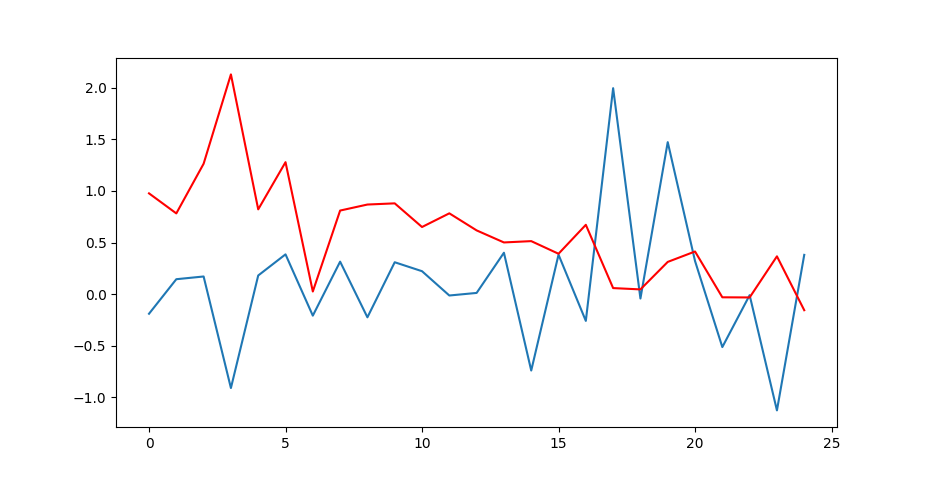
\includegraphics[width=1\textwidth] {foolad_prophet.png}
\caption{
نمودار مقایسه پیش بینی بازدهی سهم فولاد و بازدهی واقعی آن توسط مدل prophet
}
\label{foolad_prophet}$•$
\end{figure}
در شکل
\ref{foolad_prophet}
خط قرمز رنگ بازدهی پیش بینی شده توسط مدل prophet
و خط آبی رنگ بازدهی واقعی آن می باشد.
همانطور که
مشاهده می کنید، مدل خطای بالایی در پیشبینی داشته است و حتی در تشخیص
روند
\LTRfootnote{\lr{trend}}
دچار خطا شده است و الگو رو به پایین پیشبینی کرده است. طبق محاسبه ی
میانگین مربعات خطا
\LTRfootnote{\lr{mean squared error}}
به عدد نزدیک ۳ میرسیم که خطای بسیار زیادی میباشد.
\subsection{مدل LSTM}
این مدل بر پایه ی
شبکه ی عصبی بازگشتی
\LTRfootnote{\lr{Recurrent neural network}}
طراحی شده است و در مسائل الگو یابی کاربرد. جزئیات بیشتر راجع به این مدل را میتوانید در گزارش دکتر جیسون براونی
[4]
مطالعه فرمایید. از آنجایی که این مدل بسیار پیچیده است و مباحث پایه ای استفاده شده در آن خارج از مباحث داده کاوی مقدماتی می باشد، تلاشی برای تست این مدل به صورت عملی صورت نگرفت و صرفا در حد تحقیق باقی گذاشته شد.
\subsection{مدل ARIMA}
این مدل از ترکیب دو مدل AR یا همان
مدل خود‌بازنگر
\LTRfootnote{\lr{Autoregressive model}}
و MA یا همان
مدل میانگین متحرک
\LTRfootnote{\lr{Moving-average model}}
ساخته شده است.
مدل خود‌بازنگر نوعی از فرایند تصادفی می باشد و بر اساس اینکه داده ها به صورت خطی به گذشته ی خودش وابسته است و مدل MA برا اساس ارتباط بین مشاهده فعلی و خطای ایجاد شده بین پیش بینی مدل و مشاهدات قبلی کار میکند.
\par
مدل ARIMA با استفاده از ترکیب مدل AR و مدل MA  برای پیشبینی متغیر های پیجیده تر در سری های زمانی ساخته شده است .
مدل ARIMA مدلی شناخته شده و قدیمی می باشد. برای آشنایی بیشتر با مفاهیم تئوری این مدل مقاله‌ی پاول نیوبولد[5] که در سال ۱۹۸۳ به چاپ رسیده است و همچنین کتاب تحلیل سری زمانی تیسی[2] حاوی مطالب مفیدی می باشد.
این مدل دارای ۳ پارامتر می باشد که هر کدام به ترتیب مشخص کننده ی پارامتر مدل خود‌همبسته،
درجه تفاضل
\LTRfootnote{\lr{Degree of difference}}
و درجه‌ی مدل میانگین متحرک می باشد. درجه‌تفاضل تعداد دفعاتی است که باید داده با داده ی گذشته ی خود تفریق گردد تا سری زمانی
ایستا
\LTRfootnote{\lr{Stationary}}
شود. راجع به پارامتر های این مدل و نحوه ی محاسبه ی هرکدام در بخش بعد بیشتر توضیح داده شده است.
\begin{figure}[H]
\centering
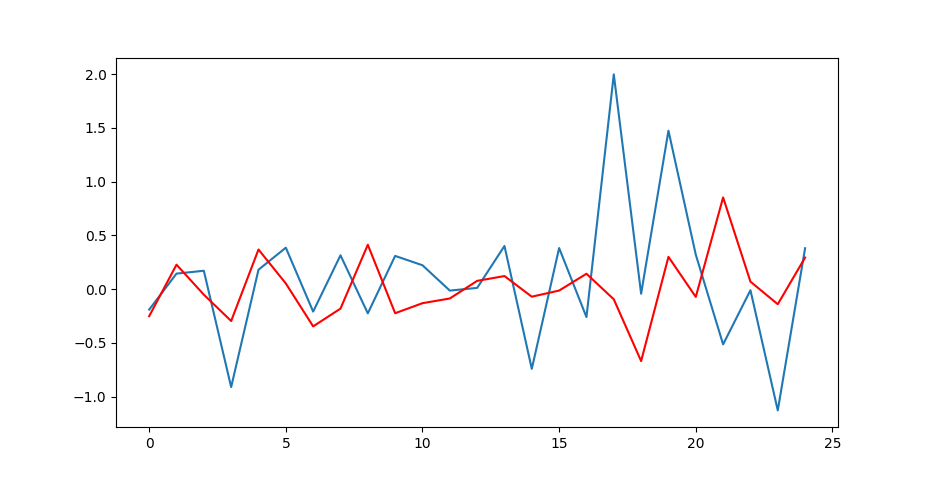
\includegraphics[width=1\textwidth] {arma1_foolad.png}
\caption{
نمودار دقت مدل رو سهم فولاد
}
\label{arma_foolad1}$•$
\end{figure}
همانطور که در شکل
\ref{arma_foolad1}
مشاهده میکنید دقت بسیار بیشتری بدست آماده است و مدل علاوه بر تشخیص صحیح روند اختلاف کمی با جواب اصلی دارد. خطا در این حالت حدود ۲۴ صدم  می باشد که به نسبت مدل prophet بسیار کمتر است.
در این نمودار خط قرمز رنگ پیش‌بینی مدل و خط آبی رنگ بازدهی سهم فولاد در ۲ سال ۲۰۲۰ و ۲۰۱۹ می باشد.
در بخش بعدی به طور کامل راجع به روند پیاده سازی مدل به کمک ARIMA صحبت خواهد شد.

\section{پیاده سازی مدل به کمک ARIMA}
بعد از نتایج مثبت اولیه که با مدل ARIMA کسب شد، این مدل به عنوان مدل پایه درنظر گرفته شد.

\subsection{تعیین پارامتر ها}
همانطور که گفته شد مدل ARIMA دارای ۳ پارامتر اصلی به ترتیب درجه ی مدل AR ، درجه تفاضل و درجه ی مدل MA می باشد. در گام نخست درجه ی تفاضل مدل را تعیین میکنیم. برا تعیین درجه ی تفاضل ابتدا وضعیت ایستایی سری زمانی را بررسی میکنیم. اگر سری زمانی ایستا باشد درجه تفاضل صفر در نظر گرفته می شود.
برای بررسی وضعیت ایستایی سری زمانی ابتدا باید نمودار سری زمانی را مورد بررسی قرار داد.
\begin{figure}[H]
\centering
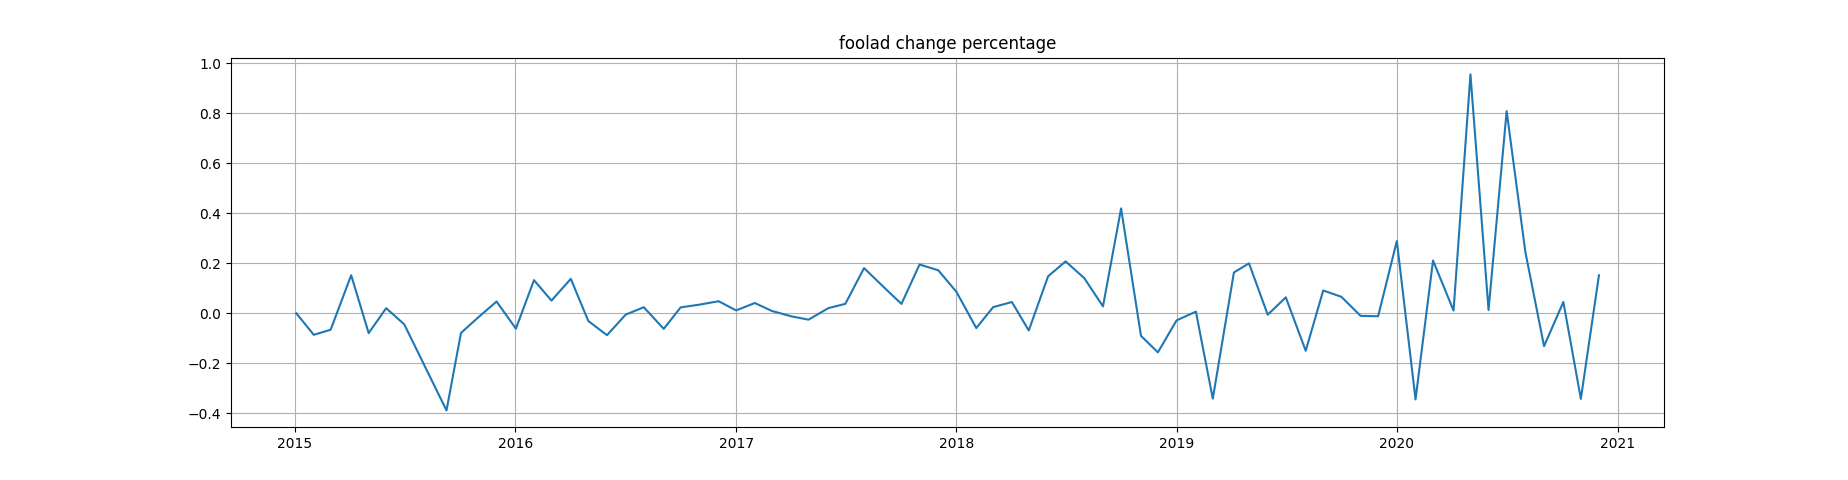
\includegraphics[width=1\textwidth] {new_foolad_stationary.png}
\caption{
نمودار نرمال شده ی بازدهی نماد فولاد
}
\label{foolad_stationary}$•$
\end{figure}
با توجه به شکل
\ref{foolad_stationary}
،
سری زمانی به طور شهودی ایستا می باشد و نمیتوان قاطعانه ایستایی سری زمانی را رد کرد به همین دلیل از
آزمون دیکی فاولر
\LTRfootnote{\lr{Dickey-Fuller test}}
جهت بررسی ایستایی مدل استفاده میکنیم.
فرض صفر در این آزمون غیر ایستا بودن سری زمانی می باشد و فرض یک ایستایی  سری زمانی می باشد.
با استفاده از تابع پایتونی adfuller آزمون فرض  بر روی سری زمانی مذکور اجرا شد و
پی-مقدار
\LTRfootnote{\lr{p-value}}
حدود ۱۳ صدم بدست آمد که با توجه به اینکه بزرگ تر از ۵ صدم می باشد شواهد کافی برای رد فرض صفر وجود ندارد پس در نتیجه سری زمانی ایستا نمی باشد.
در گام بعدی باید ایستایی سری زمانی با درجه تفاضل ۱ مورد بررسی قرار گیرد.
ازین رو با استفاده از تابع diff سری زمانی جدیدی که حاصل اختلاف هر عضو با عضو قبلی میباشد را تشکیل میدهیم و همین آزمون را مجددا روی آن اجرا میکنیم. در این آزمون پی-مقدار عددی نزدیک صفر می شود و از آنجایی که کمتر از ۵ درصد می باشد میتوانیم به این نتیجه برسیم که سری زمانی بدست آمده ایستا می باشد و میتوانیم درجه تفاضل را برای مدل ۱ در نظر بگیریم.
\par
برای تعیین پارامتر های مدل های MA و AR از نمودار های ACF  و نمودار های
PACF استفاده شده است و
به کمک توابع پایتونی plot\_acf و plot\_pacf  نمودار های مذکور ترسیم شده اند.
\begin{figure}[H]
\centering
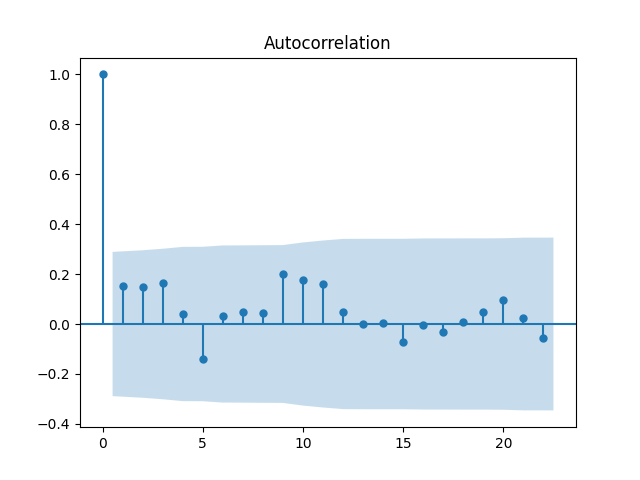
\includegraphics[width=1\textwidth] {acf.png}
\label{acf}$•$
\caption{
نمودار ACF سری زمانی نماد فولاد
}
\end{figure}

\begin{figure}[H]
\centering
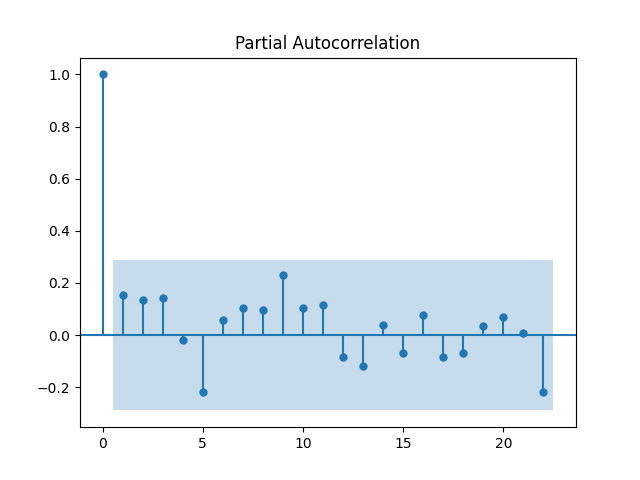
\includegraphics[width=1\textwidth] {pacf.png}
\caption{
نمودار PACF سری زمانی نماد فولاد
}
\label{pacf}$•$
\end{figure}
از نمودار
PACF جهت تعیین پارامتر مدل AR استفاده شده است
همانطور که در نمودار PACF مشخص است از اولین
لگ
\LTRfootnote{\lr{Lag}}
به بعد شاهد
برش
\LTRfootnote{\lr{Cut off}}
هستیم و همه ی نقاط در ناحیه ی آبی رنگ  که
ناحیه معناداری
\LTRfootnote{\lr{Significance area}}
نام دارد قرار دارند
با توجه به این موضوع نتیجه میگیریم که مدل روی این سری زمانی اصلا درجه‌ی مدل AR ندارد.
\par
برای تعیین پارامتر مدل MA از نمودار  ACF استفاده می کنیم
همانطور که در نمودار ACF مشخص است از اولین تاخیر شاهد برش هستیم و در ناحیه معناداری قرار میگیریم پس
نتیجه می‌شود که مدل برای این سری زمانی درجه ی MA هم ندارد.
با تکرار تمامی فرایند های بالا برای سهم های دیگر مثل اخابر و خودرو نتیجه مشابهی بدست می آید.
با توجه به اینکه نه پارامتر AR داریم نه پارامتر
MA
نتیجه میگیریم که
این دسته سری زمانی ها همگی
نویز سفید
\LTRfootnote{White noise}
هستند و نمیتوانیم با استفاده از مدل AR و مدل MA  پیش بینی خیلی دقیقی ازین سری زمانی ها داشته باشیم و مدل ARIMA هم به طبع صرفا یک مدل تفاضل گیر ساده خواهد شد و تعیین پارامتر های بهینه برای مدل ARIMA کار ساده ای نخواهد بود.
در بخش بعدی سعی میشود با اثر دهی بقیه پیشگو ها و بررسی حالت های مختلف برای پارامتر مدل ARIMA به بهترین دقت ممکن برای پیشبینی برسیم.

\subsection{اثردهی پیشگو ها}
همانطور که گفته شده است هدف، پیشبینی قیمت سهم به کمک تاریخچه‌ی خود سهم و پیشگوهای اقتصادی ذکر شده می باشد. سری زمانی هر سهم حاوی اطلاعات تاریخچه ی سهم می باشد که با وارد کردن سری زمانی به مدل، این اطلاعات در دسترس مدل قرار میگیرند ولی برای شاخص های های اقتصادی نیاز می باشد که اطلاعات این پیشگو ها به نحوی در اختیار مدل قرار بگیرند.
مدل ARIMA یک سری زمانی اضافه تحت عنوان
متغیر بیرونی
\LTRfootnote{\lr{Exogenous variables}}
در حین آموزش و پیشبینی دریافت میکند و به عنوان پیشگو اثر گذاری متغییر دریافتی را با سری زمانی اصلی که دریافت کرده بررسی میکند و در پیشبینی سری زمانی اعمال میکند.
در پیاده سازی پایتون،
این متغییر را با عنوان
exog
دریافت میکند که معادل آن در زبان R ،
xreg می باشد.
\par
در پیاده سازی پایتون ARIMA ،مدل فقط یک سری زمانی تحت عنوان متغییر بیرونی دریافت میکند و در صورت وجود چندین پیشگو رسیدگی به این موضوع به عهده ی استفاده کننده می‌باشد.
برای حل این چالش در این پروژه از ترکیب خطی بازگشت پذیر سری های زمانی پیشگو های اقتصادی استفاده شده است. بدین شکل که از ترکیب خطی سری زمانی نرمال شده ی قیمت دلار ، شاخص تورم و نقدینگی یک سری زمانی جدیدی بدست آمده است و به مدل داده شده است. از آنجایی که با نرمال سازی انجام شده واحد و مقیاس همه ی پیشگو های اقتصادی یکسان شده است این نوع ترکیب خطی از نظر علمی صحیح می باشد و کافی است ضرایب هر شاخص به طور صحیحی انتخاب شود.
با توجه به جدول
\ref{table}
و خروجی اولیه مدل ترکیب خطی زیر به عنوان متغیر بیرونی به مدل تحویل داده شد.
\begin{equation*}
0.5 * dollar + 0.5 * inflation - 0 * cash_values
\end{equation*}
در فصل بعدی نتایج بدست آمده ازین مراحل مورد بررسی قرار خواهد گرفت.

\chapter{ تحلیل نتایج و جمع بندی}
\section{نتایج بدست آمده از مدل ARIMA}
ابتدا نتایج بدست آمده از مدل را مشاهده کنیم و در آخر تحلیل نتایج را ببینیم.
دو حالت برای انجام تست روی مدل امکان پذیر بود. در هر دو حالت ابتدا داده به دو قسمت آموزشی و آزمایشی تقسیم میشود که در تست های انجام شده ی ما ۶۶ درصد داده ها از ابتدای سری زمانی به عنوان داده ی آموزشی انتخاب شدند و ما بقی به عنوان داده ی آزمایشی انتخاب شدند.
حالت اول برای تست به این روش عمل میکردیم که مدل با توجه به کل داده های آزمایشی بعلاوه ی داده هایی که خودش آن ها را پیش بینی کرده آموزش داده شود و نقطه ی بعدی را پیش بینی کند و به همین ترتیب جلو برود.
حالت دوم این است که در هر مرحله مقدار واقعی عضوی که مدل پیشبینی کرده است را به عنوان مشاهده به مجموعه داده های آموزشی اضافه کنیم و مدل مرحله ی بعدی را پیشبینی کند و به همین ترتیب پیش برویم.
ما در تمام تست ها از حالت اول استفاده کردیم و در بخش تحلیل بیشتر راجع به تفاوت این دو روش صحبت خواهد شد.
\subsection{نتایج عملی تست }
چند نمونه از نتایج به دست آمده توسط مدل طراحی شده در ادامه آمده است.
\begin{figure}[H]
\centering
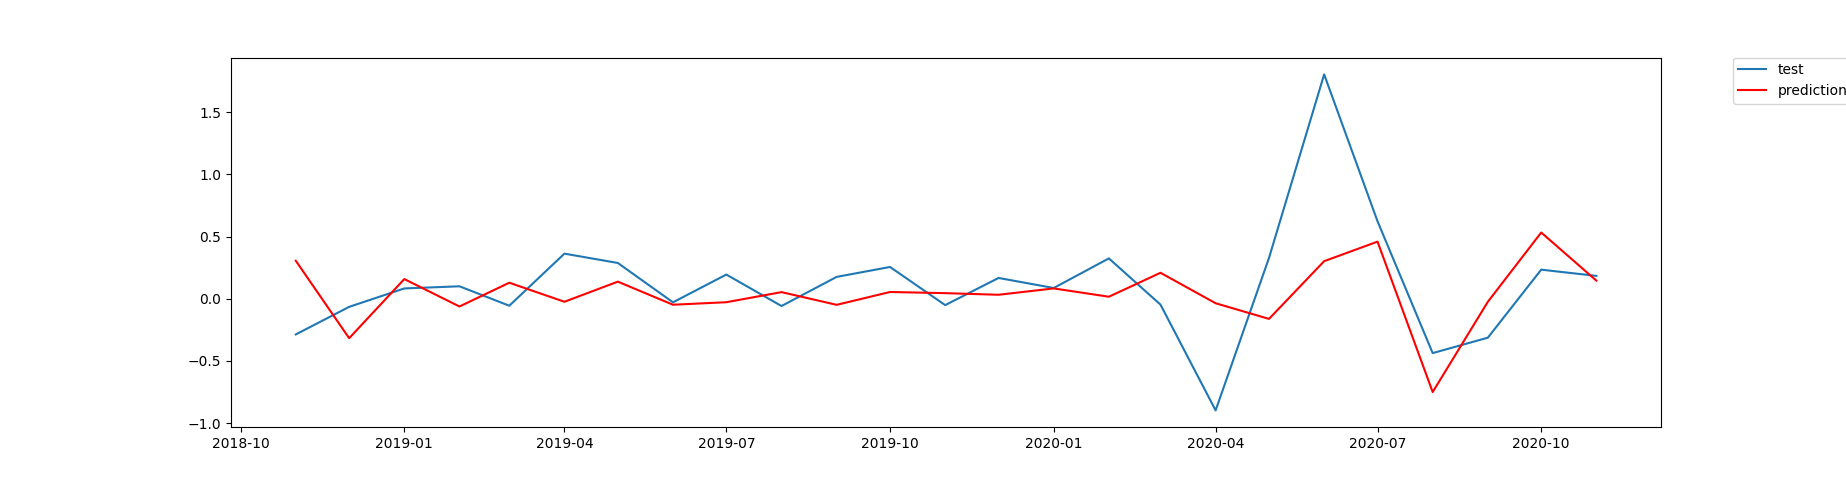
\includegraphics[width=1\textwidth] {foolad3_arima.png}
\label{foolad3_arima}$•$
\caption{
نمودار دقت مدل روی سهم خودرو با پارامتر های (۲،۱،۲)
}
\end{figure}
\begin{figure}[H]
\centering
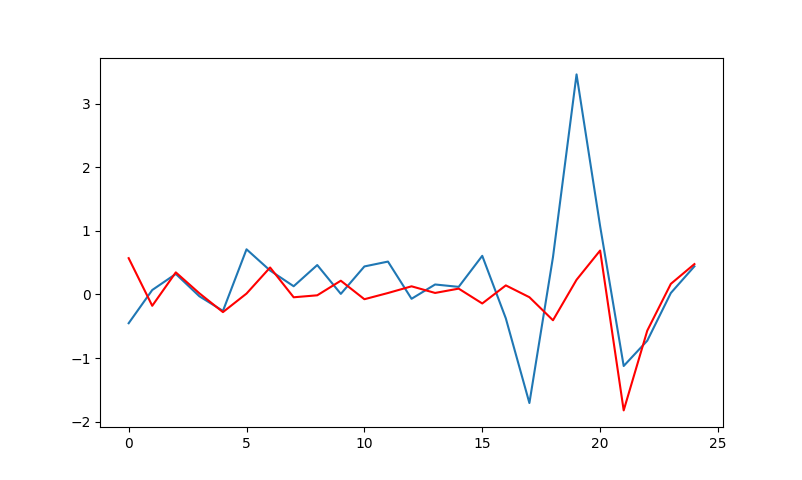
\includegraphics[width=1\textwidth] {khodro1_arima.png}
\label{khodro1_arima}$•$
\caption{
نمودار دقت مدل رو سهم خودرو با پارامتر های (۳،۰،۴)
}
\end{figure}

\begin{figure}[H]
\centering
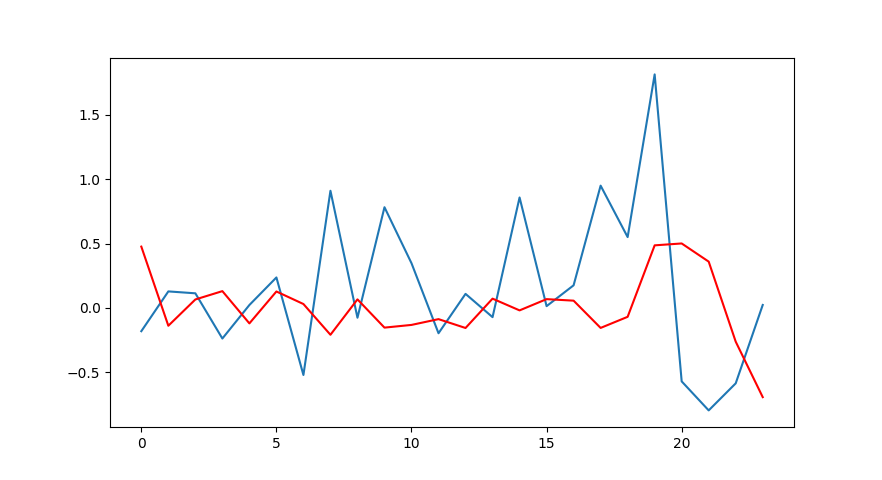
\includegraphics[width=1\textwidth] {akhaber1_arima.png}
\label{akhaber1_arima}$•$
\caption{
نمودار دقت مدل رو سهم اخابر با پارامتر های (۳،۰،۴)
}
\end{figure}

\begin{figure}[H]
\centering
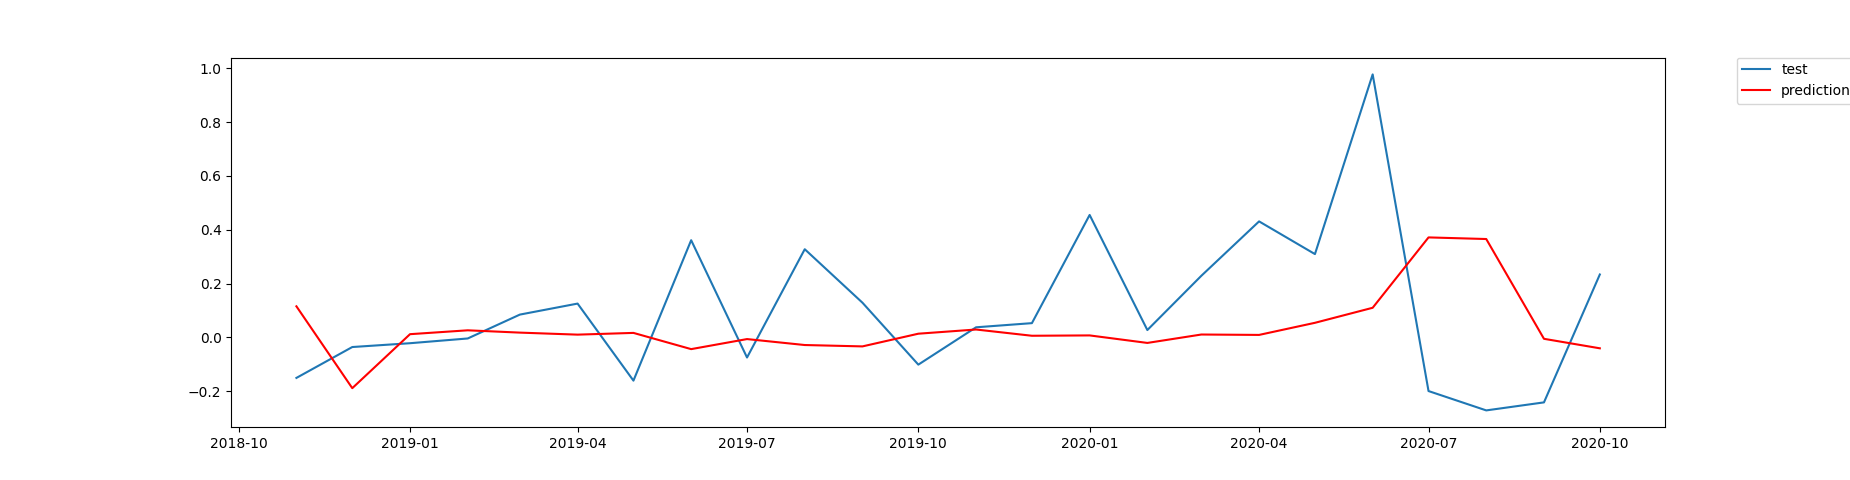
\includegraphics[width=1\textwidth] {foolad2_arima.png}
\caption{
نمودار دقت مدل رو سهم اخابر با پارامتر های (۲،۰،۰)
}
\label{akhaber2_arima}$•$
\end{figure}

\subsection{تحلیل و جمع بندی}
همانطور که مشاهده می شود مدل در شروع کار دقت بهتری دارد و در ادامه رفته رفته از دقت آن کم میشود. علت این اتفاق این است که از روشی برای آزمایش و تست مدل استفاده میکنیم که پیشبینی خود مدل را به عنوان مشاهده جدید به مدل می دهیمی و از آنجایی که این پیشبینی خطا دارد رفته رفته خطا به نقاط جلو تر بازنشر میشود و خطای نقاط جلوتر بیشتر میشود ولی با توجه به اینکه این روش در دنیای واقعی بیرون، عملی تر و ساده تر است نسبت به روش دوم و دید بلند مدت تری ارائه می دهد ترجیح دادیم مدلمان را با توجه به این روش بهینه کنیم.
در شکل
\ref{akhaber2_arima}
همانطور که مشاهده میکنید پارامتر مدل میانگین متحرک را برابر صفر قرار دادیم و مدل صرفا یه مدل ساده ی خودهمبسته شد و دقت نهایی کاهش پیدا کرد.
\par
در گام اول تست، بدون در نظر گرفتن نمودار های ACF و PACF و صرفا با آزمون و خطا
سعی شد که به بهترین دقت برسیم، سپس به کمک نمودار های نام برده شده سعی کردیم پارامتر های بهینه برای مدل ARIMA را بدست آوریم که با شکست مواجه شدیم در نتیجه مججدا به گام اول بازگشتیم و سعی کردیم به کمک آزمون و خطا و یا استفاده از تابع
auto\_arima
که با بررسی حالت های مختلف سعی میکند به بهترین پارامتر ممکن برسد،
به بهترین دقت برسیم.
چند نمونه از نتایج بدست آمده در جدول
\ref{table2}
آمده است.
\par
همانطور که مشاهده می‌شود برای سهم های مختلف پارامتر های مختلفی بهترین دقت را ارائه میدهند و قانون کلی برای تمامی سهم ها نمی توان ارائه کرد.
\par
نکته ای که در آخر لازم به ذکر می باشد این است که تاکنون مدل های بسیاری برای پیش بینی قیمت سهم ها ارائه شده است ولی هیچ کدام به گونه ای دارای دقت نبوده اند که برای سرمایه گزاری امن پیشنهاد شوند. عوامل بسیار زیادی بر قیمت سهم تاثیر گذار هستند که از چشم مدل ها مخفی می مانند، از جمله عملکرد شرکت ها که توسط کامپیوتر خیلی قابل پیش بینی نمی باشد.
\begin{table}[]
\begin{latin}
\centering
\begin{tabular}{|l|l|l|l|}
\hline
        & foolad & akhaber & khodro \\ \hline
(0,1,0) & 0.325  & 0.330   & 0.477  \\ \hline
(0,1,2) & 0.263  & 0.258   & 0.374  \\ \hline
(1,1,0) & 0.267  & 0.304   & 0.534  \\ \hline
(3,1,3) & 0.241  & 0.266   & 0.343  \\ \hline
(1,1,1) & 0.272  & 0.261   & 0.445  \\ \hline
(1,1,2) & 0.272  & 0.268   & 0.356  \\ \hline
(2,1,2) & 0.264  & 0.272   & 0.346  \\ \hline
(2,1,0) & 0.255  & 0.316   & 0.407  \\ \hline
\end{tabular}
\end{latin}
\caption{MSE}
\label{table2}
\end{table}


\chapter*{واژه‌نامه فارسی به انگلیسی}
مدل میانگین متحرک همبسته یکپارچه
\dotfill \lr{ARIMA model} \\
زبان برنامه نویسی پایتون
\dotfill \lr{Python programming language} \\
گیت
\dotfill \lr{Git} \\
پیشگو
\dotfill \lr{Predictor} \\
تورم
\dotfill \lr{Inflation} \\
نقدینگی
\dotfill \lr{Cash} \\
تاریخچه قیمت
\dotfill \lr{Price history} \\
سری زمانی
\dotfill \lr{Time series} \\
قیمت پایانی
\dotfill \lr{Closing price} \\
داده ی گم شده
\dotfill \lr{Missing data} \\
جاینهی آخرین مشاهده
\dotfill \lr{Last observation carried forward} \\
نموداراسکتر
\dotfill \lr{Scatter plot} \\
خصیصه
\dotfill \lr{Feature} \\
مدل جمعی
\dotfill \lr{Additive model} \\
رگرسیون ناپارامتری
\dotfill \lr{Nonparametric regression} \\
فصلی بودن
\dotfill \lr{Seasonality} \\
روند
\dotfill \lr{Trend} \\
میانگین مربعات خطا
\dotfill \lr{Mean squared error} \\
شبکه عصبی بازگشتی
\dotfill \lr{Recurrent neural network} \\
مدل خود همبسته
\dotfill \lr{Autoregressive model} \\
مدل میانگین متحرک
\dotfill \lr{Moving-average model} \\
درجه تفاضل
\dotfill \lr{Degree of difference} \\
آزمون دیکی فاولر
\dotfill \lr{Dickey-Fuller test} \\
پی-مقدار
\dotfill \lr{P-value} \\
تاخیر
\dotfill \lr{Lag} \\
برش
\dotfill \lr{Cut off} \\

\chapter*{مراجع}
\begin{latin}
[1] Larose D.T. and Larose C.D. (2014) Discovering knowledge in data: an introduction to data mining (Second edition). John Wiley \& Sons.
\newline
\newline
[2] Ruey S. Tsay, “Analysis of Financial Time Series, 3rd Edition”, WILEY, 2010.
\newline
\newline
[3] Time Series Data Analysis For Stock Market Prediction Using Data Mining Techniques With R, by Mahantesh Angadi
\newline
\newline
[4] https://machinelearningmastery.com/gentle-introduction-long-short-term-memory-networks-experts/, by Jason Brownlee
\newline
\newline
[5] ARIMA model building and the time series analysis approach to forecasting, by Paul Newbold,1983
\end{latin}


\begin{latin}
\begin{abstract}
The purpose of this project is to predict the future of Tehran Stock using the history of stocks and other economic indicators such as dollar price, inflation, liquidity and etc. we tried to implement a model using data mining algorithms that can predict stock future using stock's and economic indicators history. In the first step, we collected the required data. we saved all the stocks and mentioned economic indicators from 2015 to 2020 in csv format. next step, we examined which indicators affect the stock price by drawing appropriate graphs and analyzing the indicators together then we selected the appropriate indicators. In the last step, we trained an ARIMA model to predict stock future and we tested our model.
\end{abstract}
\newpage

%Title page ---------------------------------------------
\begin{figure}
\centering
\includegraphics[height=2.5cm]{UT-Logo.pdf}
\end{figure}
\begin{center}

College of Science\\
School of Mathematics, Statistics, and Computer Science
\end{center}

\begin{center}
\huge{Analysis of Iran stock exchange using data mining algorithms}
\end{center}

\begin{center}
%%%
\end{center}

\begin{center}
\textbf{
Mohammad Hossein Khoshraftar
}
\end{center}

\begin{center}
\begin{tabular}{rr}
Supervisor: & Dr. Samaneh Eftekhari Mahabadi \\

\end{tabular}
\end{center}

\vspace{3cm}
\begin{center}
A thesis submitted to Graduate Studies Office\\
in partial fulfillment of the requirements for the degree of \\
B.Sc.in\\
 Computer Science
\end{center}

\begin{center}
July , 2021
\end{center}

%\pagestyle{empty}
\pagenumbering{}

\end{latin}

\end{document}
